\chapter{Kuhn poker experiment} \label{PLEI}

\lhead{Chapter x. \emph{Kuhn poker experiment}}
In this chapter, we will present and explain the experiment on a simplified version of poker, the Kuhn poker.
First, we will describe how we setup the neural network and how we trained it. Then we will present the result and the different metrics on how well the neural network performed. Finally, we will analyze the result and try to generalize them to any imperfect game.

\section{Setup} \label{kuhnexperiment:setup}

\subsubsection{environment}
We created a Kuhn poker environment that gives us all the necessary data to correctly feed the neural network. We have defined 3 actions possible: check, bet and fold. We have decided to regroup raise and bet in the same action "bet" to reduce the complexity. If at any time the decision-making NN predicts an incorrect action, the default action "bet" or "check" would be done.

\subsubsection{NN}
We decided to first use a simple RNN for the opponent modeling, you can find more information about the specific input of this NN in section \ref{methodology:opponent-modelling}, see figure \ref{fig:opponent-modelling-nn-rnn}. We used the decision making NN describe in section \ref{methodology:descision-making}, figure \ref{fig:decision-making-nn}.

Different layers size has been tested, from 10 to 20 for the hidden layer size of the descision making NN and from 5 to 20 for the opponent modelling NN. We also tried to add an other hidden layer for both NN. activation function, and opponent model size has been tested. We did not notice any improvement while increasing the layer size above 10 for both NN.

Different activation function has been tried, linear, sigmoid and relu. The result between the sigmoid and the linear function are pretty similar. However the relu had bad performance compared to the linear.

Different opponent model size has been tested, from 5 to 20. While analyzing the neural networks we have seen that the decision making NN uses at most 5 input, the others were not impacting the decision. However it is worth to notice that due to the way our training is done, it makes sense to use a larger opponent model size because we can not except all the opponent model output to be meaningful.

Only the most successful architecture will be presented, their results will be detailed in the section \ref{kuhnexperiment:result}. The descriptions of their NN layers are detailed in table \ref{tab:nn-layer-kuhn}. The size of the input layer is defined by the environment and the opponent model size. It has been detailed in the section \ref{methodology:NN}. 

\begin{table}[ht]
\centering
\begin{tabular}{ |c|c|c| }
 \hline
 NN name & opponent-modelling NN  & descision-making NN \\ 
 \hline
 input layer & x & x \\ 
 \hline
 hidden layer & 10 & 10 \\
 activation & linear & linear \\
 \hline
 output layer & opponent model size & 3 (check, bet, fold) \\
 activation & sigmoid & softmax \\
 \hline
\end{tabular}
\caption{NN layer (kuhn poker)}
\label{tab:nn-layer-kuhn}
\end{table}

\subsection{Training}
To train the NN we have used competitive co-evolution, general information about it can be found in section \ref{methodology:competitive-co-evolution}.

We have used these strategy in the teaching set:

\begin{itemize}
    \item \textbf{Equilibrium}: playing the equilibrium strategy
    \item \textbf{Random}: playing a random action in the set of the available ones
    \item \textbf{Always bet}
    \item \textbf{Always fold}
    \item \textbf{Close Equilibrium}: playing a strategy close to the equilibrium. It select each action with a probability chosen uniformly randomly within 0.2 of the equilibrium probability. It aims to produce realistic sub-optimal opponent.
\end{itemize}

We have by default added 3 different \textit{Close Equilibrium} strategies to the teaching set. We have not used a system to dynamically add training agents to the teaching set. We are making each agent playing against each other and using a shared fitness to promote diversity (ref: \ref{LR:competitive-co-evolution}). To make the result of the games not based on cards luck, we are first making the two agents play a set of rounds. Then, we erase their memory and make them play with the opposite cards. A temporary reward is attributed, the agent winning 1, the one losing -1, then the final reward is attributed after the shared fitness calculation.

The EA has been used with these parameters. These parameters have been decided after multiple iterations, those seem to have good training performance in this context. For reference, we have put in italic the range of the values that we looked at.
\begin{itemize}
    \item population size: 20 ; \textit{10 to 25}
    \item individual kept each iteration: 5 ; \textit{2 to 5}
    \item mutation rate: 0.1 ; \textit{0.1 to 0.2}
    \item iteration: 100 ; \textit{10 to 100}
    \item number of rounds (games): 25 ; \textit{5 to 25}
\end{itemize}



\section{Result} \label{kuhnexperiment:result}
To evaluate the NN we apply the evaluation method detailed in the section \ref{requirement:evaluation}.

In this section, results of multiple NN models will be presented, the NN and EA parameters are by default the one described in the previous section \ref{kuhnexperiment:setup}.

\begin{itemize}
    \item \textbf{Classic}: No parameters changes.
    \item \textbf{More Games}: Playing 50 games per iteration (instead of 25). Only 10 individuals and 3 are kept at each iteration.
    \item \textbf{Bigger Model Size}: The opponent model size is 10 (instead of 5)
    \item \textbf{Larger Teaching Set}: Having 6 \textit{Close Equilibrium} agents in the teaching set
\end{itemize}

Due to the limited resources, the models are from a single run of the EA. For the record, one run takes approximately 2h, performances are discussed in section TODO-SECTION-SCALE-UP.

\subsection{Win rate}

In this section we will present the win rate of the different tested models against multiple strategies, the choices of these strategies are detailed in the section \ref{requirement:evaluation}.  We made the agents played together 500 games, erased their memory then played another 500 games with the opposite cards. You can find the results in the table \ref{tab:reward-kuhn}.

It is worth mentioning that the \textit{Close Equilibrium} strategy during the evaluation is not one of the training set.

\begin{table}[h]
\resizebox{\textwidth}{!}{
\begin{tabular}{ |c|c|c|c|c|c|c|c| }
 \hline
 Opponent Model & E & Close E & Random & Always Bet & Always Fold & TBR & Random then TBR \\ 
 \hline
 Classic & 0.001 & 0.053 & 0.202 & 0.293 & 0 & -0.182 & -0.139 \\
 \hline
 More Games & 0.006 & 0.001 & 0.312 & 0.200 & 0.646 & -0.175 & -0.116 \\ 
 \hline
 Bigger Model Size & -0.02 & 0.027 & 0.309 & 0.180 & 0.106 & -0.087 & -0.065 \\
 \hline
 Larger Teaching Set & 0.001 & 0.054 & 0.196 & 0.350 & 0 & -0.172 & -0.120 \\
 \hline
 Equilibrium & 0 & 0.007 & 0.150 & 0.104 & 0.238 & -0.125 & -0.118 \\
 \hline
\end{tabular}
}
\caption{Win rate in mbb/hand of the opponent model against evaluation opponent for the kuhn poker (Equilibrium has been shortened to E and true best response to TBR)}
\label{tab:reward-kuhn}
\end{table}
\subsubsection{Sub-optimal opponent exploitation}

We can see that the model \textit{Classic} have really good performance against \textit{Close Equilibrium} (0.054) compared to the equilibrium (0.007). It demonstrates the capacity of the NN model to exploit sub-optimal opponent.

In the study \citep{ganzfried2015safe}, they have an agent playing the best response according to the opponent model that they use for reference to demonstrate how unsafe it is. This algorithm have similar result as \textbf{Classic} regarding the \textit{Close Equilibrium} (called sophisticated static in this study). However, the main difference is that the model \textit{Classic} is less exploitable. Indeed comparing the difference between equilibrium and the algorithm for the random then TBR (called dynamic in the other study). It gives us 0.021 for \textit{Classic} and 0.085 for the best response in the study. To sum up, using NN we are capable of achieving as good results as algorithms fully committed to opponent exploitation while being less exploitable.

\subsubsection{Impact of training}

We can notice that model \textit{Classic} and \textit{Larger Teaching Set} perform poorly against always fold, an opponent that is supposed to be easily exploitable. We can assume it is linked to the way NN are trained. In competitive EA with shared fitness, it is likely that a strategy exploiting a stronger opponent (always bet) will have a better fitness compared to exploiting a simple opponent (always fold). Polishing the EA training would likely improve and stabilize the results over multiple runs.

In addition EA are known to be stochastic, meaning that the results are hard to be predictable. That is because of the random elements such as the initialisation, selection and mutation. To have a good and predictable result, you are likely going to need to run multiple times the process and select the best of them.

\subsubsection{Exploitability}

The true best response help understands how much an algorithm is exploitable, it has access to every player's cards and plays the best response every time. It is not an absolute metric but highlight if an algorithm is likely to be exploitable.

An interesting thing about the \textit{Bigger Model Size} model result is that it performs better than the equilibrium against the \textit{TBR} and \textbf{Random then TBR}. Both of these strategies are "cheating" by having access to the opponent private information to produce the true best response. We can assume that the NN is noticing that the opponent is particularly good and decide to play super safe minimizing the loss. It demonstrates that using NN to model the opponent is not easily exploitable. Most important, it demonstrates that it can reduce the exploitability if the opponent is aware of a part of your private information.

In real-life use cases, it is frequent that some of your private information is known by the opponent. For example, if you are negotiating a deal, the person may know the budget of your company while you think it is private information.

\subsection{Reward over time}

In this section, we will present the interesting plots of the reward over time for different models.

The different plots showcase in this section are based on 1000 played games. It is worth to note that the EA training has been run having only 25 games played between each agent. Using a different scale (from 25 to 1000) demonstrate how the NN model handle keeping an opponent model through more game than usual.

\begin{figure}[ht]
    \centering
    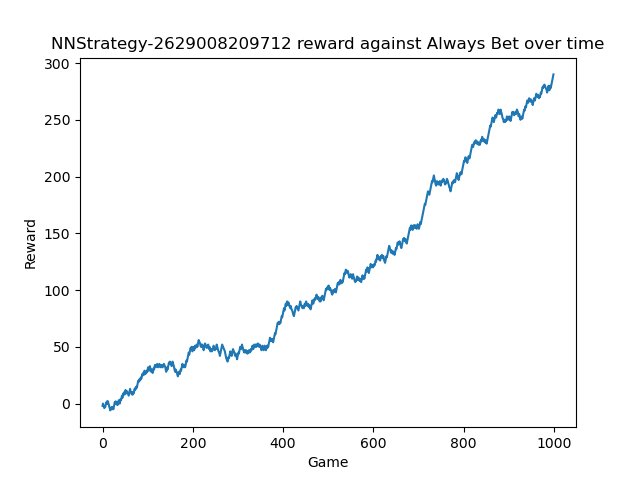
\includegraphics[width=0.7\textwidth]{Figures/out-plots/kuhn/larger-teaching-set/reward-against-Always Bet.png}
    \caption{Model Larger Teaching Set, reward against Always Bet over time}
    \label{fig:kuhn:larger-teaching-set-always-bet}
\end{figure}

In figure \ref{fig:kuhn:larger-teaching-set-always-bet}, you can see that at the very beginning, the reward is neither increasing nor decreasing. Then after some games, we can assume that the NN draws a model of the opponent, and start to exploit it by having a relatively stable increase of the reward.

\begin{figure}[ht]
    \centering
    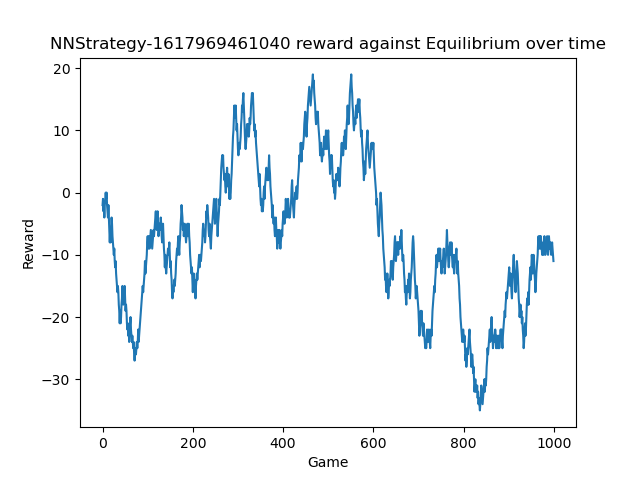
\includegraphics[width=0.7\textwidth]{Figures/out-plots/kuhn/more-games/reward-against-Equilibrium.png}
    \caption{Model More Games, reward against Equilibrium over time}
    \label{fig:kuhn:more-games-equilibrium}
\end{figure}

In figure \ref{fig:kuhn:more-games-equilibrium}, you can see that there is not a straight tendency of increasing or decreasing. It's what you expect from a game against two opponents without net exploitation. It demonstrates the ability of the model to not fall into a wrong interpretation or at least recover/correct the opponent model.

\subsection{Input impact on the NN} \label{kuhnexperiment:result:input-impact}

We have measured the impact of each input to every output of the neural network to determine how much the input is taken into consideration in the decision. To do that we used SHAP \citep{shap}, a game-theoretic approach to explain the output of any machine learning model. On the plots, inputs are ordered by impact. Each blue dot represents the impact (positive or negative) of one input for one activation.

\begin{figure}[ht]
    \centering
    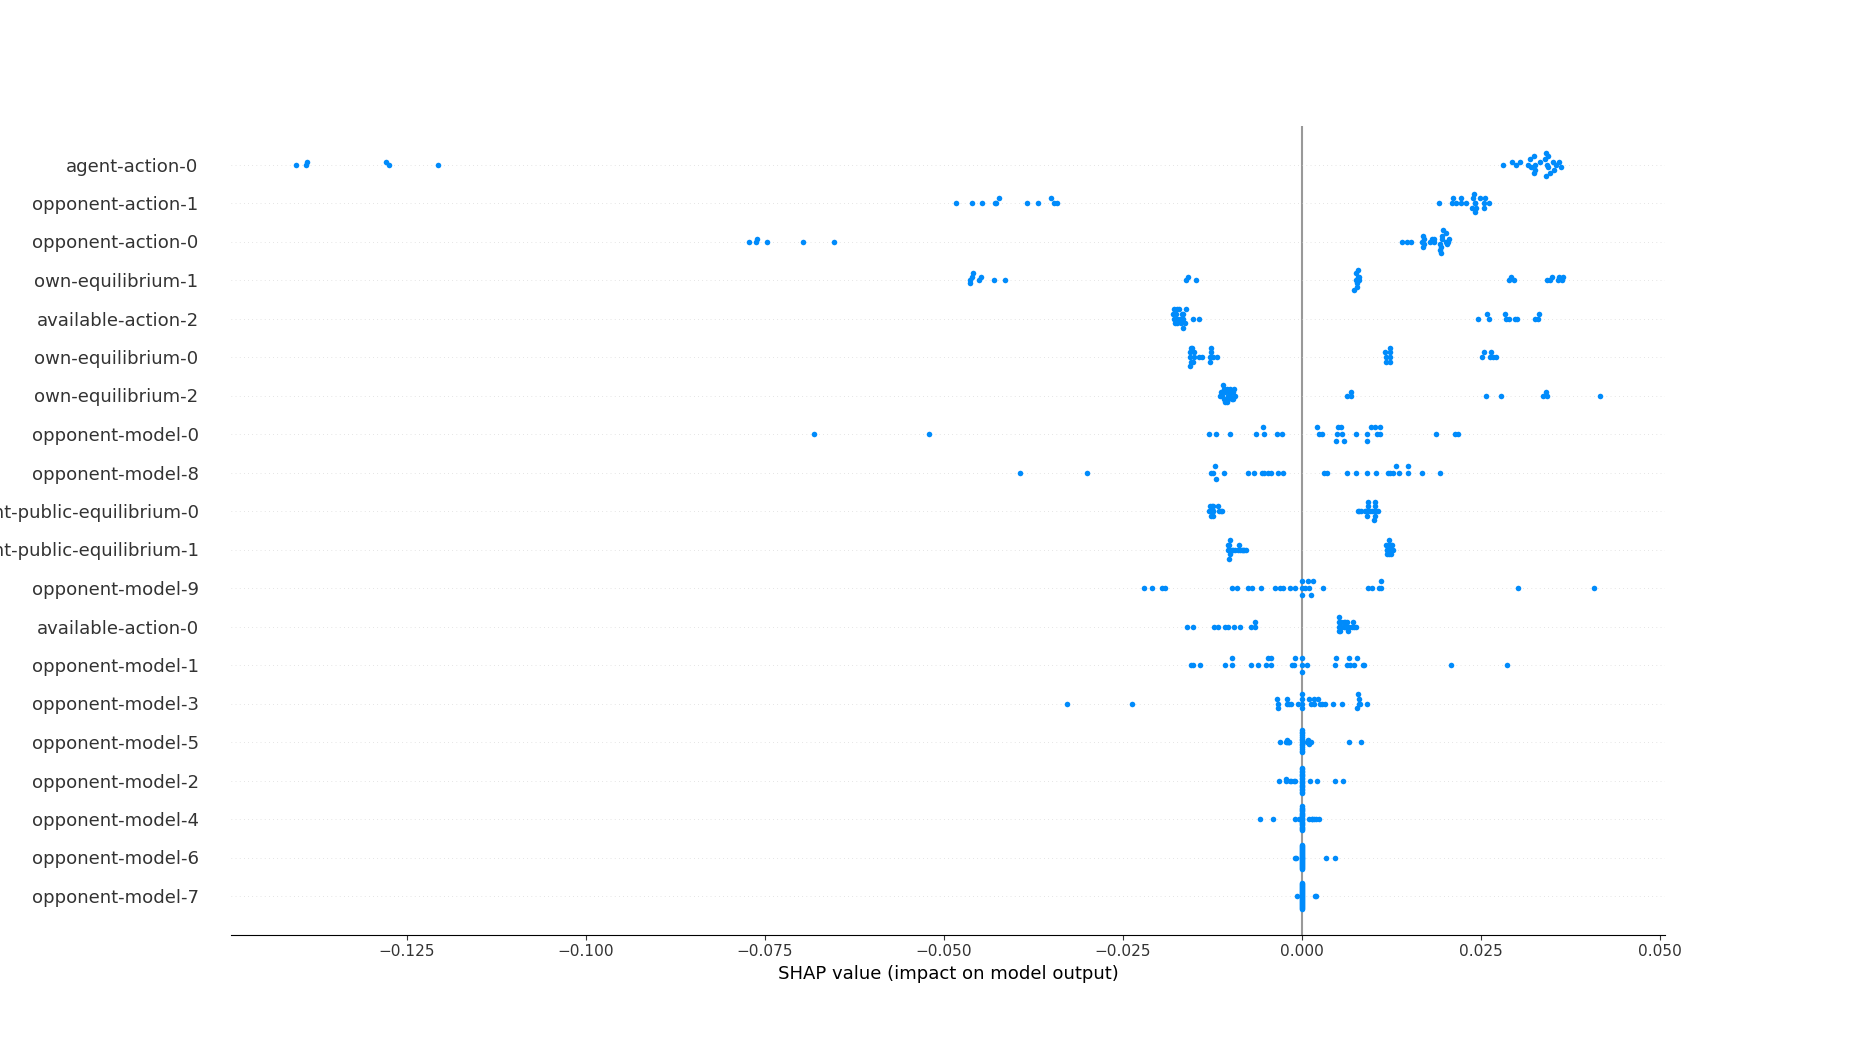
\includegraphics[width=1\textwidth]{Figures/out-plots/kuhn/bigger-model/action-check-input-impact.png}
    \caption{Bigger Model Size, input impact for the check action}
    \label{fig:kuhn:bigger-model-impact-check}
\end{figure}

\begin{figure}[ht]
    \centering
    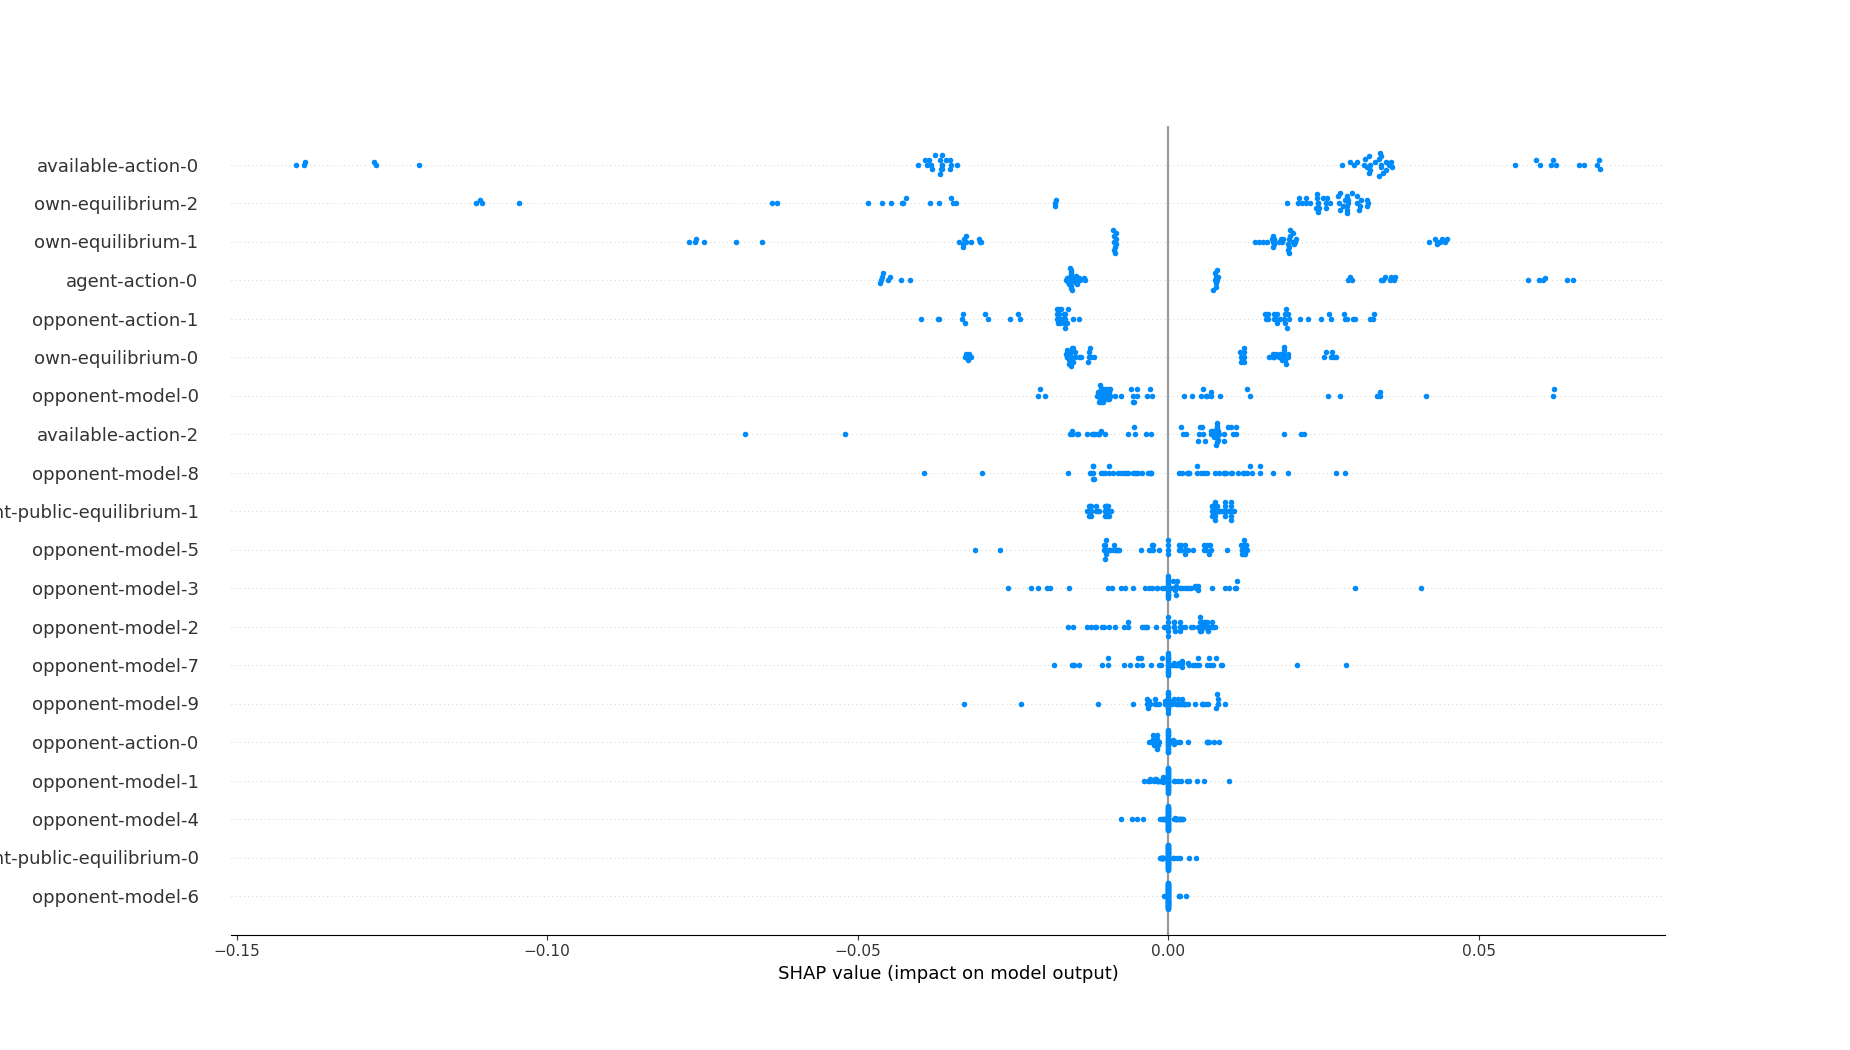
\includegraphics[width=1\textwidth]{Figures/out-plots/kuhn/bigger-model/action-bet-input-impact.png}
    \caption{Bigger Model Size, input impact for the bet action}
    \label{fig:kuhn:bigger-model-impact-bet}
\end{figure}

For the model \textit{Bigger Model Size}, we can see that on the opponent-model-0 input is part of the most impacting input for the bet and check action, figure \ref{fig:kuhn:bigger-model-impact-check} and \ref{fig:kuhn:bigger-model-impact-bet}. It demonstrates that the NN relies on the opponent model to take its decision.

\begin{figure}[ht]
    \centering
    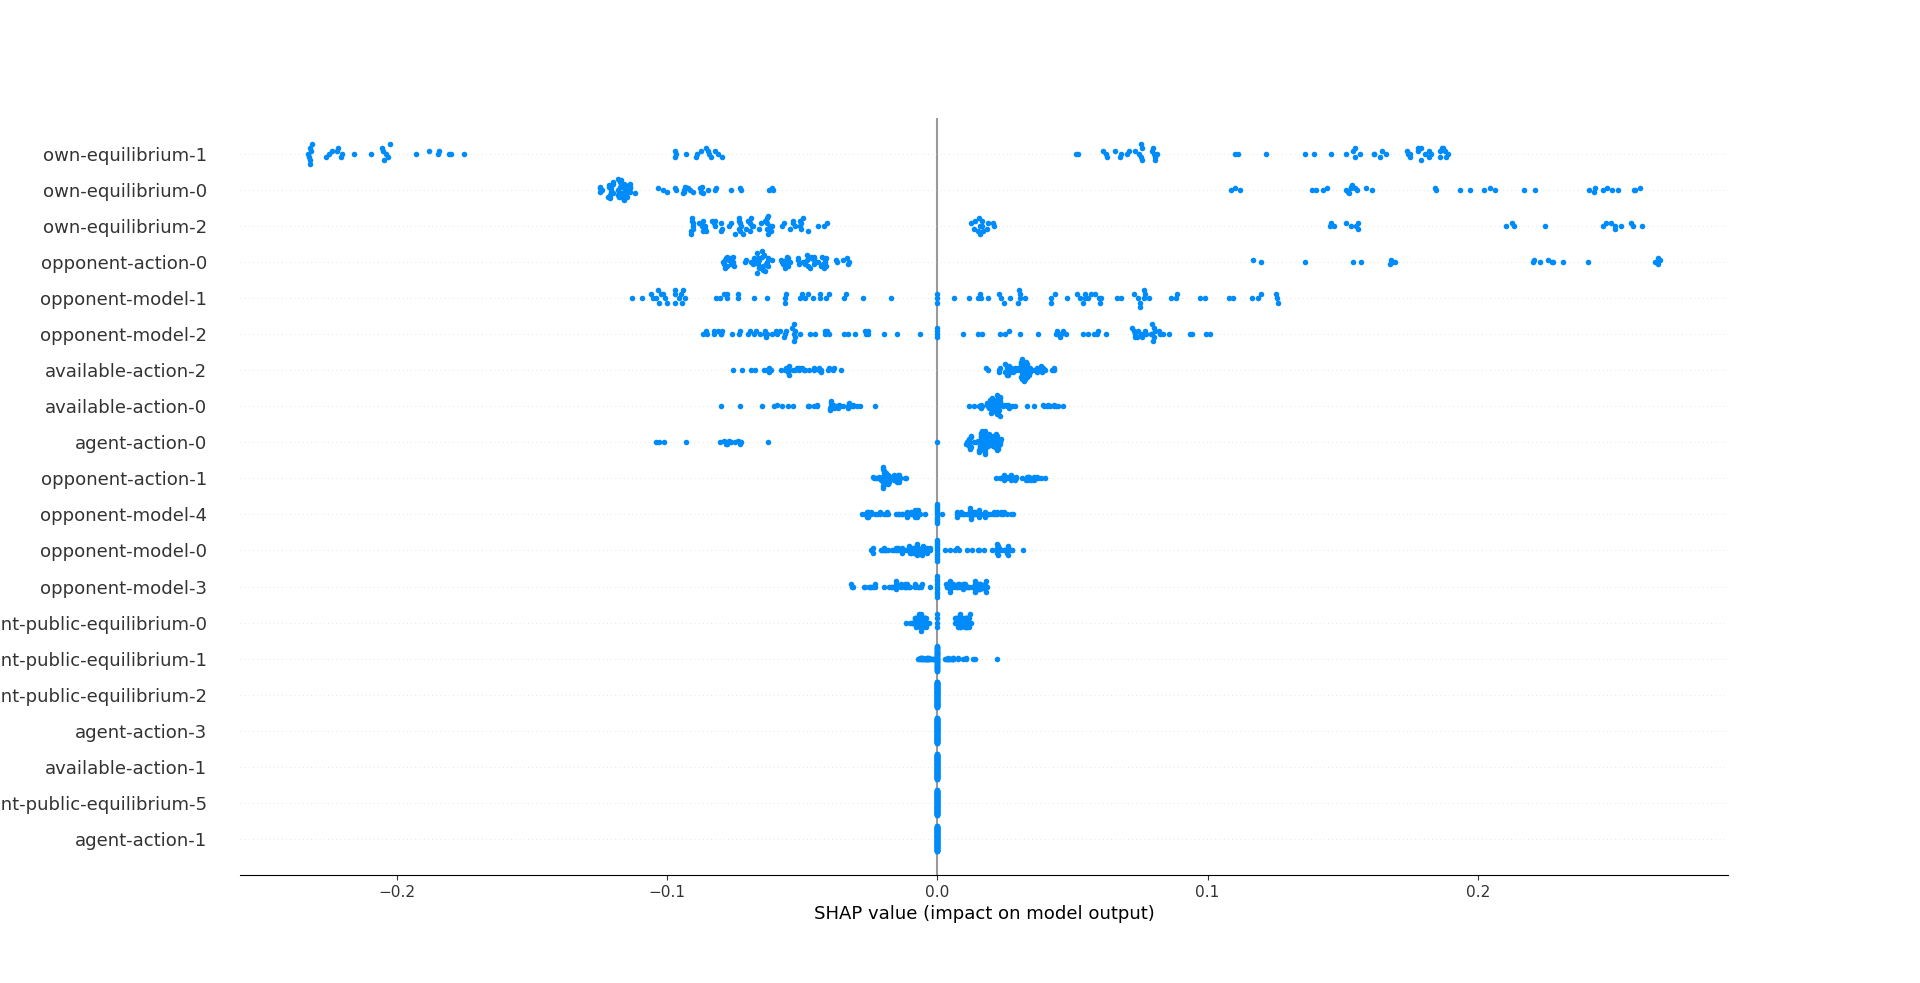
\includegraphics[width=1\textwidth]{Figures/out-plots/kuhn/A/action-fold-input-impact.png}
    \caption{Bigger Model Size, input impact for opponent-model-0}
    \label{fig:kuhn:bigger-model-impact-opponent-model-0}
\end{figure}

For the model \textit{Bigger Model Size} we can also analyze how the "opponent-model-0" is made by analyzing the opponent model NN, figure \ref{fig:kuhn:bigger-model-impact-opponent-model-0}. We can see that the most used inputs are the game outcome, the first opponent action, and the first agent action. Interpreting the purpose of this opponent model output is hazardous because NN are complex. For example, a possible analysis is that this part of the opponent model aims to define if the opponent is often winning when he is betting.

\section{Analysis}

\subsection{Approximation or incorrect Equilibrium}

During the development, I had a bug that allowed cards to be draw multiple times. It was possible to have the player one king and the second with another king (which is not possible in the Kuhn poker). So it makes the equilibrium incorrect. Even if the equilibrium was incorrect it managed to overcome this and exploit the different strategies. This means that using NN to exploit opponents in imperfect games using this NN architecture can manage and overcome incorrect or approximated equilibrium.

It is worth mentioning that the performances are likely to be degraded because the NN will need to learn the game. Indeed it will likely rely on the game history such as the previous action instead of relying on the equilibrium.

Obviously, this bug has been fixed and the presented result in the previous section are with the correct version.

\section{Conclusion}

With this Kuhn poker experiment, we can draw some general conclusions about opponent exploitation with neural networks in imperfect games.

We have demonstrated the capacity of a NN to model and exploit an opponent.

We have seen that it is way less exploitable than other existing algorithms used to model the opponent. Some models were having really good exploitability results, even better than equilibrium. Demonstrating that they were able to reduce their exploitability if the opponent knew some private information.

We have also highlighted the importance of the training phase and its impact on the quality of the model.

To conclude using NN to model opponents achieves as good results as existing algorithms while being way less exploitable than them.
